\documentclass[
]{jss}

\usepackage[utf8]{inputenc}

\providecommand{\tightlist}{%
  \setlength{\itemsep}{0pt}\setlength{\parskip}{0pt}}

\author{
Sahir Bhatnagar *\\McGill University \And Maxime Turgeon *\\University of Manitoba \AND Jesse Islam\\McGill University \And James Hanley\\McGill University \And Olli Saarela\\University of Toronto
}
\title{\pkg{casebase}: An Alternative Framework For Survival Analysis}

\Plainauthor{Sahir Bhatnagar *, Maxime Turgeon *, Jesse Islam, James Hanley, Olli Saarela}
\Plaintitle{casebase: An Alternative Framework For Survival Analysis}
\Shorttitle{\pkg{casebase}: An Alternative Framework For Survival Analysis}

\Abstract{
The abstract of the article. * joint co-authors
}

\Keywords{keywords, not capitalized, \proglang{Java}}
\Plainkeywords{keywords, not capitalized, Java}

%% publication information
%% \Volume{50}
%% \Issue{9}
%% \Month{June}
%% \Year{2012}
%% \Submitdate{}
%% \Acceptdate{2012-06-04}

\Address{
    Sahir Bhatnagar *\\
  McGill University\\
  1020 Pine Avenue West Montreal, QC, Canada H3A 1A2\\
  E-mail: \email{sahir.bhatnagar@mail.mcgill.ca}\\
  URL: \url{http://sahirbhatnagar.com/}\\~\\
      Maxime Turgeon *\\
  University of Manitoba\\
  186 Dysart Road Winnipeg, MB, Canada R3T 2N2\\
  E-mail: \email{max.turgeon@umanitoba.ca}\\
  URL: \url{https://maxturgeon.ca/}\\~\\
      Jesse Islam\\
  McGill University\\
  1020 Pine Avenue West Montreal, QC, Canada H3A 1A2\\
  E-mail: \email{jesse.islam@mail.mcgill.ca}\\
  
      James Hanley\\
  McGill University\\
  1020 Pine Avenue West Montreal, QC, Canada H3A 1A2\\
  E-mail: \email{james.hanley@mcgill.ca}\\
  URL: \url{http://www.medicine.mcgill.ca/epidemiology/hanley/}\\~\\
      Olli Saarela\\
  University of Toronto\\
  Dalla Lana School of Public Health, 155 College Street, 6th floor,
  Toronto, Ontario M5T 3M7, Canada\\
  E-mail: \email{olli.saarela@utoronto.ca}\\
  URL: \url{http://individual.utoronto.ca/osaarela/}\\~\\
  }

% Pandoc header

\usepackage{amsmath} \usepackage{longtable} \usepackage{graphicx} \usepackage{tabularx} \usepackage{float} \usepackage{booktabs} \usepackage{makecell} \DeclareUnicodeCharacter{2500}{-}

\begin{document}

\hypertarget{case-study-3support-data}{%
\section{Case study 3--SUPPORT Data}\label{case-study-3support-data}}

In the first two case studies, we described the basic functionalities of
the \pkg{casebase} package: creating population-time plots, fitting
parametric models for hazard functions, and estimating the corresponding
cumulative incidence curves. In the next two case studies, we explore
more advanced features.

For the third case study, we will introduce regularization into the
estimation of the hazard function. This can be performed using a
combination of case-base sampling and regularized logistic regression.
To demonstrate this capability, we examine the Study to Understand
Prognoses Preferences Outcomes and Risks of Treatment (SUPPORT) dataset
\citep{knaus1995support}. The SUPPORT dataset tracks death for
individuals who are considered seriously ill within a hospital.
Imputation was conducted using the \pkg{mice} package in \proglang{R}
with default settings \citep{mice}. Before imputation, there were a
total of 1000 individuals and 35 variables. charges, Totcst, totmcst and
sfdm2 were removed as they are response variables we are not interested
in for the sake of this analysis. After imputation, we have 690
individuals. We lose individuals due to coliniarity between variables,
preventing imputation. If a pair of covariates are deemed colinear to a
certain degree, they are excluded from any imputations. Here, only edu
income avtisst* race ph* glucose* adlp* were imputed. Of these 690
individuals, 66.09\% experienced the event of interest. A description of
each variable can be found in Table \ref{tab:support1} and a breakdown
of each categorical variable in Table \ref{tab:support2}. The original
data was obtained from the Department of Biostatistics at Vanderbilt
University. The imputed dataset is available as part of the
\pkg{casebase} package.

\begin{table}[ht]
\centering
\begin{tabular}{ccccc}
\hline
\textbf{Name} & \textbf{Labels}                          & \textbf{Levels} & \textbf{Storage} & \textbf{NAs} \\
\hline
age           & Age                                      &                 & double           & 0            \\
death         & Death at any time up to NDI date:31DEC94 &                 & double           & 0            \\
sex           &                                          & 2               & integer          & 0            \\
hospdead      & Death in Hospital                        &                 & double           & 0            \\
slos          & Days from Study Entry to Discharge       &                 & double           & 0            \\
d.time        & Days of Follow-Up                        &                 & double           & 0            \\
dzgroup       &                                          & 8               & integer          & 0            \\
dzclass       &                                          & 4               & integer          & 0            \\
num.co        & number of comorbidities                  &                 & double           & 0            \\
edu           & Years of Education                       &                 & double           & 202          \\
income        &                                          & 4               & integer          & 349          \\
scoma         & SUPPORT Coma Score based on Glasgow D3   &                 & double           & 0            \\
charges       & Hospital Charges                         &                 & double           & 25           \\
totcst        & Total RCC cost                           &                 & double           & 105          \\
totmcst       & Total micro-cost                         &                 & double           & 372          \\
avtisst       & Average TISS, Days 3-25                  &                 & double           & 6            \\
race          &                                          & 5               & integer          & 5            \\
meanbp        & Mean Arterial Blood Pressure Day 3       &                 & double           & 0            \\
wblc          & White Blood Cell Count Day 3             &                 & double           & 24           \\
hrt           & Heart Rate Day 3                         &                 & double           & 0            \\
resp          & Respiration Rate Day 3                   &                 & double           & 0            \\
temp          & Temperature (Celsius) Day 3              &                 & double           & 0            \\
pafi          & PaO2/(.01*FiO2) Day 3                    &                 & double           & 253          \\
alb           & Serum Albumin Day 3                      &                 & double           & 378          \\
bili          & Bilirubin Day 3                          &                 & double           & 297          \\
crea          & Serum creatinine Day 3                   &                 & double           & 3            \\
sod           & Serum sodium Day 3                       &                 & double           & 0            \\
ph            & Serum pH (arterial) Day 3                &                 & double           & 250          \\
glucose       & Glucose Day 3                            &                 & double           & 470          \\
bun           & BUN Day 3                                &                 & double           & 455          \\
urine         & Urine Output Day 3                       &                 & double           & 517          \\
adlp          & ADL Patient Day 3                        &                 & double           & 634          \\
adls          & ADL Surrogate Day 3                      &                 & double           & 310          \\
sfdm2         &                                          & 5               & integer          & 159          \\
adlsc         & Imputed ADL Calibrated to Surrogate      &                 & double           & 0           
\end{tabular}
\caption{A description of each variable in the SUPPORT dataset.}
\label{tab:support1}
\end{table}

\begin{table}[ht]
\centering
\begin{tabular}{cc}
\hline
\textbf{Variable} & \textbf{Levels}                      \\
\hline
sex      & female                                        \\
         & male                                          \\
dzgroup  & ARF/MOSF w/Sepsis                             \\
         & COPD                                          \\
         & CHF                                           \\
         & Cirrhosis                                     \\
         & Coma                                          \\
         & Colon Cancer                                  \\
         & Lung Cancer                                   \\
         & MOSF w/Malig                                  \\
dzclass  & ARF/MOSF                                      \\
         & COPD/CHF/Cirrhosis                            \\
         & Coma                                          \\
         & Cancer                                        \\
income   & under \$11k                                   \\
         & $11-$25k                                      \\
         & $25-$50k                                      \\
         & \textgreater{}\$50k                           \\
race     & white                                         \\
         & black                                         \\
         & asian                                         \\
         & other                                         \\
         & hispanic                                      \\
sfdm2    & no(M2 and SIP pres)                           \\
         & adl\textgreater{}=4 (\textgreater{}=5 if sur) \\
         & SIP\textgreater{}=30                          \\
         & Coma or Intub                                 \\
         & \textless{}2 mo. follow-up                   
\end{tabular}
\caption{A description of each level within each categorical variable in the dataset.}
\label{tab:support2}
\end{table}

As before, the first step is to visualize the incidence density. The
population-time plot for the SUPPORT data appears in Figure
\ref{fig:support-poptime}.

\begin{CodeChunk}
\begin{figure}

{\centering 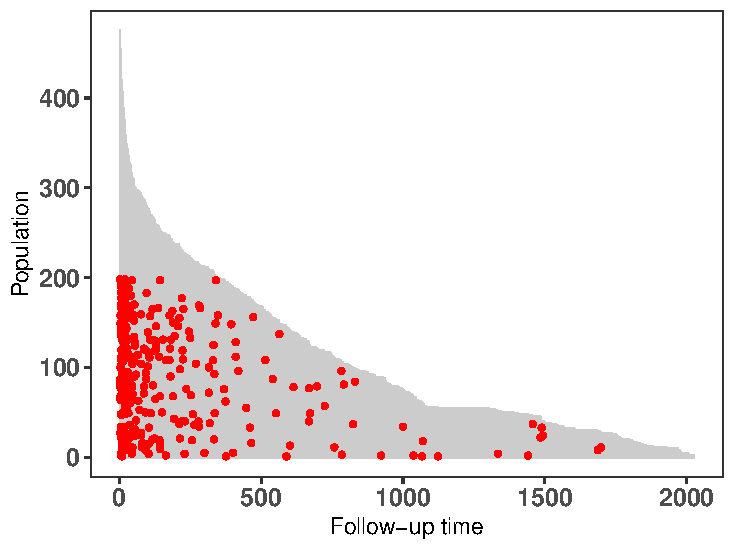
\includegraphics{../figures/support-poptime-1} 

}

\caption{\label{fig:support-poptime} Population-time plot for the SUPPORT data. Red points represent the case series. The gray space demonstrates the base series.}\label{fig:support-poptime}
\end{figure}
\end{CodeChunk}

Before we proceed with the analysis, we first remove hospital death as a
covariate, as this is directly informative of death. All covariates will
be used to estimate the hazard function. The hazard function will be
used to estimate the cumulative incidence of each individual in the
study. Then, the average cumulative incidience curve for all
observations will be used for our comparison.

Our main objective is to compute the absolute risk of death for a given
set of covariates, using regularization when fitting our model. First,
we fit a smooth hazard to the data using a weibull distribution. As
casebase makes use of the glmnet package, we interact with the
fitsmoothhazard.fit function using a matrix interface, where y contains
the time and event variables and x contains all other variables we would
like to include in the model. For the SUPPORT dataset, all factor
variables were converted into indicator variables. Here, we used lasso
penalization by setting alpha to 1.

\begin{CodeChunk}

\begin{CodeInput}
R> 
R> cb.ModelInter=casebase::fitSmoothHazard.fit(x,y,family="glmnet",time="d.time",event="death",
R+                                        formula_time = ~log(d.time),alpha=1,ratio=ratio)
\end{CodeInput}
\end{CodeChunk}

Then, we take our model and use the \texttt{absoluteRisk} function to
integrate and retrieve our cumulative incidence curves.

We will compare this curve to a regularized version of cox regression,
and a kaplan-meier survival curve. The cox regression absolute risk
curve with lasso penalization required two extra steps to retrieve.
Coxnet from the glmnet package has tools to fit a regularized cox model,
but requires a survival object skeleton of the selected variables, so
that the survival package tools can be used to retrive the absolute
risk. We handle this by fitting a regularized cox model with the glmnet
package, and a cox model from the survival package with the selected
variables from the regularized fit. This second model serves as a
skeleton that permits the use of survival package functions. The
coefficients from the regularized model will replace the coefficients in
our skeleton. the resulting model will have the correct coefficients
when integrating, but will have an incorrect standard error. For the
purposes of this case study, we are only interested in the absolute risk
curve itself and not the standard error.

We used the survival package to calculate the kaplan-meier absolute risk
function.

\begin{CodeChunk}

\begin{CodeInput}
R> #creating a surv object to be used to fit an unadjusted absolute risk curve.
R> # (Kaplan-Meier risk curve)
R> km <- survival::Surv(time = completeData$d.time, event = completeData$death)
R> abKm<-survival::survfit(km~1,type='kaplan-meier',conf.type='log')
\end{CodeInput}
\end{CodeChunk}

Now that our three absolute risk functions have been calculated, we
compare them all in Figure \ref{fig:abSC}. Both coxnet and casebase
decrease the absolute risk by the end of the study, in comparison to
kaplan-meier.

\begin{CodeChunk}

\begin{CodeInput}
R> # A plot to compare all three Absolute risk (Commulative Incidence)
R> plot(cbCIAve[,1],cbCIAve[,2],type='l',col="black",lwd=3,main="Support- CaseBase vs. Cox+glmnet vs KM Absolute Risk Curves",xlab="Survival-Time",ylab="Cumulative Incidence",ylim=c(0,1),xlim=)
R> lines(abCF,col="red",fun="event",lwd=3,conf.int = FALSE)
R> lines(abKm ,col="Blue",fun="event",lwd=3,conf.int = FALSE)
R> legend("bottomright", 
R+        legend = c( "Casebase (Lasso+linear)","semi-parametric (Cox)+glmnet","KM curve"), 
R+        col = c("black","red","Blue"),
R+        lty = c(1, 1, 1), 
R+        bg = "gray90")
\end{CodeInput}
\begin{figure}

{\centering 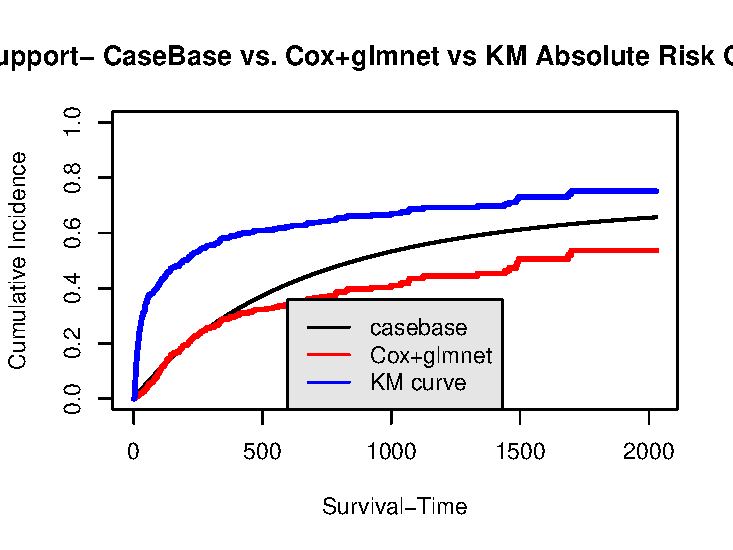
\includegraphics{../figures/abSupportComparison-1} 

}

\caption{\label{fig:abSC} Compares regularized casebase in black, regularized cox in red and Kaplan meier in blue.}\label{fig:abSupportComparison}
\end{figure}
\end{CodeChunk}

\begin{CodeChunk}

\begin{CodeInput}
R> 
R> #get covariates excluding d.time
R> estimatescb=setDT(as.data.frame(coef(cb.Model)[-c(1,2),1]), keep.rownames = TRUE)[]
R> estimatescb$Model="casebase"
R> colnames(estimatescb)<-c("Coefs","Estimate","Model")
R> estimatescox=setDT(as.data.frame(coef(coxNet)[-c(1),1]), keep.rownames = TRUE)[]
R> estimatescox$Model="Cox"
R> colnames(estimatescox)<-c("Coefs","Estimate","Model")
R> estimates=rbind(estimatescb, estimatescox)
R> estimates$Estimate[estimates$Estimate==0]=NA# make it so unchosen covariates appear empty
R> library(ggstance)# for vertical dodge
R>   ggplot(estimates, aes(x = Estimate, y = Coefs, color = Model)) +
R>         geom_segment(aes(x = 0, y = Coefs, xend = Estimate, yend = Coefs),size=0.5 ) +
R>         geom_point(position=ggstance::position_dodgev(height=0.2))
R> 
\end{CodeInput}
\end{CodeChunk}

\bibliography{references.bib}


\end{document}

